\section{Származtatás, absztrakt osztályok, interfészek}

\subsection{Származtatás, védett tagok, virtuális függvények}

\begin{frame}
    \small
    Feladat: készítsünk osztályokat egy átlagos alkalmazott, és egy programozó bérének kiszámítására!
    \begin{center}
        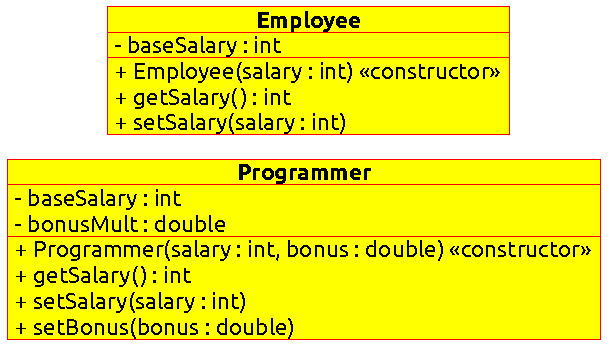
\includegraphics[scale=0.75]{inheritance01.eps} \\
        \tiny A program \hiv{\href{https://www.visual-paradigm.com/guide/uml-unified-modeling-language/uml-class-diagram-tutorial/}{UML osztálydiagram}}ja.
    \end{center}
\end{frame}

\begin{frame}
    \begin{columns}[T]
        \column{.4\textwidth}
            \begin{exampleblock}{\textattachfile{inheritance01.cpp}{Employee}}
                \vspace{-.2cm}
                \fontsize{7}{8} \selectfont
                \lstinputlisting[language=C++,linerange={3-15},numbers=left,firstnumber=3]{inheritance01.cpp}
                \vspace{-.2cm}
            \end{exampleblock}
        \column{.6\textwidth}
            \begin{exampleblock}{\textattachfile{inheritance01.cpp}{Programmer}}
                \vspace{-.2cm}
                \fontsize{7}{8} \selectfont
                \lstinputlisting[language=C++,linerange={17-34},numbers=right,firstnumber=17]{inheritance01.cpp}
                \vspace{-.2cm}
            \end{exampleblock}
    \end{columns}
\end{frame}

\begin{frame}[fragile]
    \begin{exampleblock}{\textattachfile{inheritance01.cpp}{main()}}
        \footnotesize
        \lstinputlisting[language=C++,linerange={36-41},numbers=left,firstnumber=36]{inheritance01.cpp}
    \end{exampleblock}
    \begin{block}{Kimenet}
        \footnotesize
        \vspace{-.3cm}
        \begin{verbatim}
300000
750000
        \end{verbatim}
        \vspace{-.6cm}
    \end{block}
\end{frame}

\begin{frame}
    Probléma:
    \begin{itemize}
        \item Hasonló feladatok következménye: kódismétlés (a programozó az alkalmazott egy speciális esete).
    \end{itemize}
    Megoldás:
    \begin{itemize}
        \item Származtatás/öröklés (inheritance)
        \item Ősosztály/szülő osztály (superclass, base class) $\to$ \texttt{Employee}
        \item Leszármazott/származtatott/gyerek osztály (subclass, derived class) $\to$ \texttt{Programmer}
    \end{itemize}
\end{frame}

\begin{frame}
    \begin{center}
        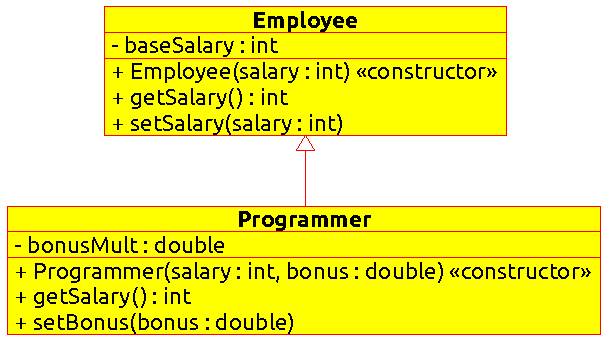
\includegraphics[scale=0.75]{inheritance02.eps}
      \end{center}
\end{frame}

\begin{frame}
    \begin{itemize}
        \item A leszármazottakban (felül)definiáljuk azokat a függvényeket, amik másképpen fognak viselkedni (\texttt{getSalary()}), mint az ősben vagy teljesen hiányoztak (\texttt{setBonus()}).
        \item Minden más átöröklődik, kivéve a konstruktort. (Ettől még nem feltétlenül elérhetők ezek a leszármazottban! $\to$ \texttt{private})
        \item Ősosztálytól örökölt tagok inicializálása a leszármazott dolga, pl. az ős konstruktorának felhasználásával a taginicializáló listán. Ennek hiányában a fordító az ős alapértelmezett konstruktorát hívja.
    \end{itemize}
\end{frame}

\begin{frame}
    \begin{columns}[T]
        \column{.4\textwidth}
            \begin{exampleblock}{\textattachfile{inheritance02.cpp}{Employee}}
                \vspace{-.2cm}
                \fontsize{7}{8} \selectfont
                \lstinputlisting[language=C++,linerange={3-15},numbers=left,firstnumber=3]{inheritance02.cpp}
                \vspace{-.2cm}
            \end{exampleblock}
        \column{.6\textwidth}
            \begin{exampleblock}{\textattachfile{inheritance02.cpp}{Programmer}}
                \vspace{-.2cm}
                \fontsize{7}{8} \selectfont
                \lstinputlisting[language=C++,linerange={17-34},numbers=right,firstnumber=17]{inheritance02.cpp}
                \vspace{-.2cm}
            \end{exampleblock}
    \end{columns}
\end{frame}

\begin{frame}[fragile]
    \begin{exampleblock}{\textattachfile{inheritance02.cpp}{main()}}
        \footnotesize
        \lstinputlisting[language=C++,linerange={36-40},numbers=left,firstnumber=36]{inheritance02.cpp}
    \end{exampleblock}
    \begin{block}{Kimenet}
        \footnotesize
        \vspace{-.3cm}
        \begin{verbatim}
300000
750000
        \end{verbatim}
        \vspace{-.6cm}
    \end{block}
\end{frame}

\begin{frame}[fragile]
    \begin{exampleblock}{\textattachfile{inheritance02.cpp}{main()}}
        \footnotesize
        \lstinputlisting[language=C++,linerange={42-48},numbers=left,firstnumber=42]{inheritance02.cpp}
    \end{exampleblock}
    \begin{block}{Kimenet}
        \footnotesize
        \vspace{-.3cm}
        \begin{verbatim}
300000
300000
        \end{verbatim}
        \vspace{-.6cm}
    \end{block}
\end{frame}

\begin{frame}
    Probléma:
    \begin{itemize}
        \item Az ős privát tagjainak elérése körülményes a leszármazottból.
    \end{itemize}
    Megoldás:
    \begin{itemize}
        \item A védett (\texttt{protected}) tagok elérhetők a saját osztályukban és minden leszármazottban.
        \item Származtatásnál is használható ez és a \texttt{private} kulcsszó, bár szinte mindig \texttt{public}-ot használunk, azaz nem korlátozzuk tovább az öröklött láthatósági kategóriákat.
    \end{itemize}
\end{frame}

\begin{frame}
    \begin{center}
        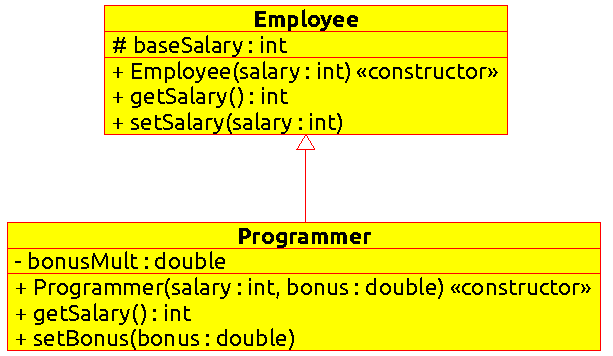
\includegraphics[scale=0.75]{inheritance03.eps}
      \end{center}
\end{frame}

\begin{frame}
    \begin{center}
        \begin{tabular}{ p{4cm}|p{3cm}|p{3cm} } 
        Származtatás módja & \multicolumn{2}{c}{Láthatóság} \\
        & ősben & leszármazottban \\
        \hline
        \texttt{public} & \texttt{public} & \texttt{public} \\ 
        & \texttt{protected} & \texttt{protected} \\ 
        & \texttt{private} & (nem érhető el) \\ 
        \texttt{protected} & \texttt{public} & \texttt{\kiemel{protected}} \\ 
        & \texttt{protected} & \texttt{protected} \\ 
        & \texttt{private} & (nem érhető el) \\ 
        \texttt{private} & \texttt{public} & \texttt{\kiemel{private}} \\ 
        & \texttt{protected} & \texttt{\kiemel{private}} \\ 
        & \texttt{private} & (nem érhető el) \\ 
        \end{tabular}
    \end{center}
\end{frame}

\begin{frame}
    \begin{description}[m]
        \item[Mikor érdemes \texttt{protected} vagy \texttt{private} származtatást végezni?] \hfill \\ Meglévő implementáció újrahasznosításánál, ha forrásban nem elérhető, de új függvényekkel (pl. más paraméterezés) kellene ellátni. 
    \end{description}
    
\end{frame}

\begin{frame}
    Probléma:
    \begin{itemize}
        \item Az ősre utaló típusú, de a leszármazott egyik példányát címző mutatóval csak az ős függvényét tudjuk hívni.
    \end{itemize}
    Megoldás:
    \begin{itemize}
        \item Amikor egy objektum tagfüggvényét hívjuk, mindig eldönthető, hogy az ős vagy a leszármazott felüldefiniált függvényéről van-e szó, és fordítási időben meghatározható annak címe (\emph{early/static bindig, korai/statikus kötés}). \\ Pl. \texttt{Programmer p(300000, 2.5); p.getSalary();} $\to$ 750000
        \item Viszont egy objektum elérhető az ős típust címző mutatóval is (biztonságos, mert a leszármazott mindennel rendelkezik, amivel az őse). A korai kötés miatt az ősben definiált függvényt tudjuk csak elérni.
    \end{itemize}
\end{frame}

\begin{frame}
    \begin{itemize}
        \item A \emph{késői/dinamikus kötés} (late/dynamic binding) hatására a fordító \emph{virtuális metódustáblát} (VMT, vtable) hoz létre, melyben a leszármazottak felüldefiniált függvényeinek címei is benne vannak, melynek segítségével az aktuális objektum típusának megfelelő változat is hívható, típuskényszerítés nélkül. \\ Pl.: \texttt{Employee* pe = new Programmer(); pe->getSalary();} $\to$ 300000
        \item C++-ban késői kötést \emph{virtuális tagfüggvényekkel} (\texttt{virtual}) hozhatunk létre.
        \item \emph{Polimorfizmus} (többalakúság): mindig az ős típusát címző mutatót használjuk, de a vele hívott tagfüggvény osztályonként eltérően működik. (A felültöltött tagfüggvények is egyfajta polimorfizmust valósítanak meg.)
    \end{itemize}
\end{frame}

\begin{frame}
    \begin{columns}[T]
        \column{.45\textwidth}
            \begin{exampleblock}{\textattachfile{inheritance03.cpp}{Employee}}
                \vspace{-.2cm}
                \fontsize{7}{8} \selectfont
                \lstinputlisting[language=C++,linerange={3-16},numbers=left,firstnumber=3]{inheritance03.cpp}
                \vspace{-.2cm}
            \end{exampleblock}
        \column{.55\textwidth}
            \begin{exampleblock}{\textattachfile{inheritance03.cpp}{Programmer}}
                \vspace{-.2cm}
                \fontsize{7}{8} \selectfont
                \lstinputlisting[language=C++,linerange={18-33},numbers=right,firstnumber=17]{inheritance03.cpp}
                \vspace{-.2cm}
            \end{exampleblock}
    \end{columns}
\end{frame}

\begin{frame}[fragile]
    \begin{exampleblock}{\textattachfile{inheritance03.cpp}{main()}}
        \footnotesize
        \lstinputlisting[language=C++,linerange={35-35},numbers=left,firstnumber=35]{inheritance03.cpp}
        \lstinputlisting[language=C++,linerange={41-46},numbers=left,firstnumber=41]{inheritance03.cpp}
    \end{exampleblock}
    \begin{block}{Kimenet}
        \footnotesize
        \vspace{-.3cm}
        \begin{verbatim}
300000
750000
        \end{verbatim}
        \vspace{-.6cm}
    \end{block}
\end{frame}

\subsection{Absztrakt osztályok}

\begin{frame}
    Induljunk ki \textattachfile{Rectangle12.cpp}{Rectangle12}-ből, majd 
    \begin{itemize}
        \item a kerület/terület lekérdezést (minden síkidomnál hasonlóan elvégezhető tevékenység) válasszuk külön a számítások elvégzésétől,
        \item a méretek legyenek módosíthatóak, és
        \item készítsünk háromszög (\texttt{Triangle}) osztályt is!
    \end{itemize}
\end{frame}    
     
\begin{frame}
    \begin{columns}[T]
        \column{.5\textwidth}
            \begin{exampleblock}{\textattachfile{Rectangle14.h}{Rectangle14.h}}
                \scriptsize
                \lstinputlisting[language=C++,linerange={4-10},numbers=left,firstnumber=4]{Rectangle14.h}
            \end{exampleblock}
        \column{.5\textwidth}
            \begin{exampleblock}{\textattachfile{Triangle14.h}{Triangle14.h}}
                \scriptsize
                \lstinputlisting[language=C++,linerange={6-11},numbers=right,firstnumber=6]{Triangle14.h}
            \end{exampleblock}
    \end{columns}
\end{frame}

\begin{frame}
    \begin{columns}[T]
        \column{.5\textwidth}
            \begin{exampleblock}{\textattachfile{Rectangle14.h}{Rectangle14.h}}
                \scriptsize
                \lstinputlisting[language=C++,linerange={11-22},numbers=left,firstnumber=11]{Rectangle14.h}
            \end{exampleblock}
        \column{.5\textwidth}
            \begin{exampleblock}{\textattachfile{Triangle14.h}{Triangle14.h}}
                \scriptsize
                \lstinputlisting[language=C++,linerange={12-23},numbers=right,firstnumber=12]{Triangle14.h}
            \end{exampleblock}
    \end{columns}
\end{frame}

\begin{frame}
    \begin{columns}[T]
        \column{.5\textwidth}
            \begin{exampleblock}{\textattachfile{Rectangle14.h}{Rectangle14.h}}
                \scriptsize
                \lstinputlisting[language=C++,linerange={23-33},numbers=left,firstnumber=23]{Rectangle14.h}
            \end{exampleblock}
        \column{.5\textwidth}
            \begin{exampleblock}{\textattachfile{Triangle14.h}{Triangle14.h}}
                \scriptsize
                \lstinputlisting[language=C++,linerange={24-34},numbers=right,firstnumber=24]{Triangle14.h}
            \end{exampleblock}
    \end{columns}
\end{frame}

\begin{frame}
    \begin{columns}[T]
        \column{.5\textwidth}
            \begin{exampleblock}{\textattachfile{Rectangle14.cpp}{Rectangle14.cpp}}
                \fontsize{7}{8} \selectfont
                \vspace{-.2cm}
                \lstinputlisting[language=C++,linerange={3-6},numbers=left,firstnumber=3]{Rectangle14.cpp}
                \lstinputlisting[language=C++,linerange={13-19},numbers=left,firstnumber=13]{Rectangle14.cpp}
                \lstinputlisting[language=C++,linerange={29-31},numbers=left,firstnumber=29]{Rectangle14.cpp}
                \vspace{-.2cm}
            \end{exampleblock}
        \column{.5\textwidth}
        \begin{exampleblock}{\textattachfile{Triangle14.cpp}{Triangle14.cpp}}
            \fontsize{7}{8} \selectfont
            \vspace{-.2cm}
            \lstinputlisting[language=C++,linerange={3-6},numbers=right,firstnumber=3]{Triangle14.cpp}
            \lstinputlisting[language=C++,linerange={18-24},numbers=right,firstnumber=18]{Triangle14.cpp}
            \lstinputlisting[language=C++,linerange={34-38},numbers=right,firstnumber=34]{Triangle14.cpp}
            \vspace{-.2cm}
        \end{exampleblock}
    \end{columns}
\end{frame}

\begin{frame}[fragile]
    \begin{exampleblock}{\textattachfile{main14.cpp}{main14.cpp}}
        \vspace{-.2cm}
        \fontsize{7}{8} \selectfont
        \lstinputlisting[language=C++,linerange={2-15},numbers=left,firstnumber=2]{main14.cpp}
        \vspace{-.2cm}
    \end{exampleblock}
    \begin{block}{Kimenet}
        \vspace{-.4cm}
        \fontsize{7}{8} \selectfont
        \begin{verbatim}
Rectangle #1 Area: 2 Perimeter: 6
Rectangle #2 Area: 6 Perimeter: 10
Rectangle #3 Area: 12 Perimeter: 14
        \end{verbatim}
        \vspace{-.6cm}
    \end{block}
\end{frame}

\begin{frame}[fragile]
    \begin{exampleblock}{\textattachfile{main14.cpp}{main14.cpp}}
        \vspace{-.2cm}
        \fontsize{8}{9} \selectfont
        \lstinputlisting[language=C++,linerange={16-27},numbers=left,firstnumber=16]{main14.cpp}
        \vspace{-.2cm}
    \end{exampleblock}
    \begin{block}{Kimenet}
        \vspace{-.4cm}
        \fontsize{8}{9} \selectfont
        \begin{verbatim}
Triangle #1 Area: 6 Perimeter: 12
Triangle #2 Area: 30 Perimeter: 30
Triangle #3 Area: 84 Perimeter: 56
        \end{verbatim}
        \vspace{-.6cm}
    \end{block}
\end{frame}

\begin{frame}
    Probléma:
    \begin{itemize}
        \item Sok ismétlődő kódrészlet $\to$ szükség lenne egy általános síkidomra a származtatáshoz, de az milyen adatokkal írható le? Hogyan számolható ki pl. a kerülete?
    \end{itemize}
    Megoldás:
    \begin{itemize}
        \item \emph{Absztrakt} (abstract) osztály: csak öröklési céllal hozzák létre, nem példányosítható a nem implementált, ún. \emph{pure virtual} tagfüggvények (absztrakt metódus) miatt
        \item Ha egy absztrakt osztály kizárólag pure virtual tagfüggvényeket tartalmaz: \emph{interfész} (interface) $\to$ elvárt szolgáltatáscsomag előírására
    \end{itemize}
\end{frame}

\begin{frame}
    \begin{center}
        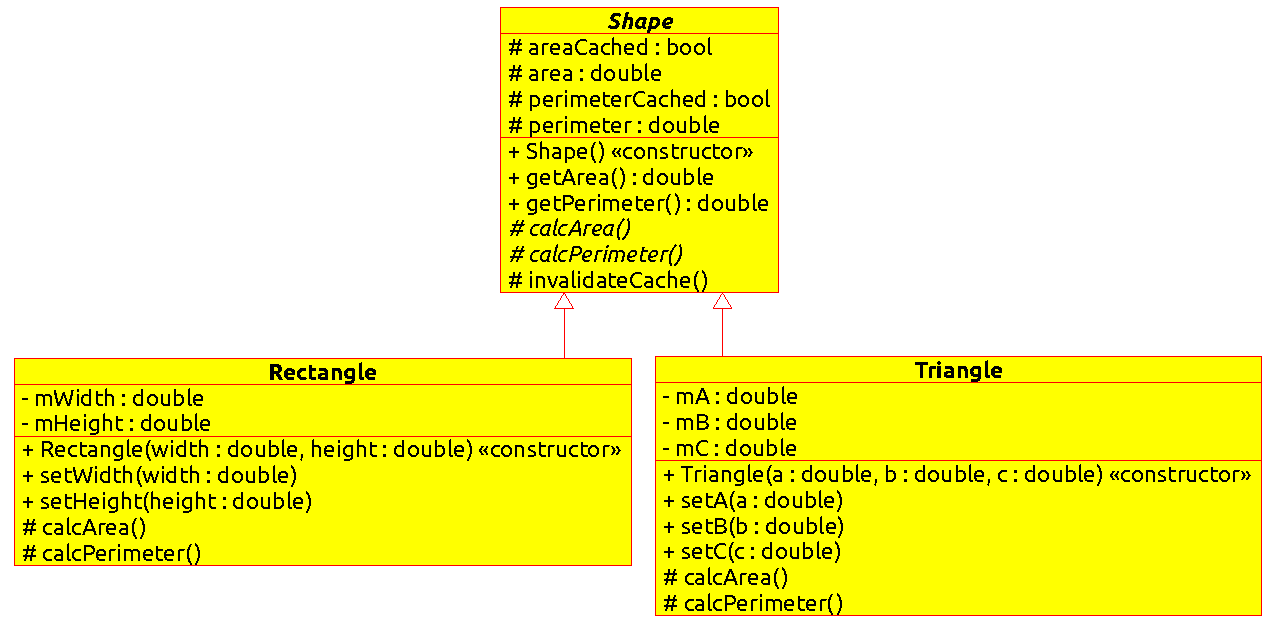
\includegraphics[scale=0.6]{Shape15.eps} \\
      \end{center}
\end{frame}

\begin{frame}
    \begin{exampleblock}{\textattachfile{Shape15.h}{Shape15.h}}
        \lstinputlisting[language=C++,linerange={4-13},numbers=left,firstnumber=4]{Shape15.h}
    \end{exampleblock}
\end{frame}

\begin{frame}
    \begin{exampleblock}{\textattachfile{Shape15.h}{Shape15.h}}
        \lstinputlisting[language=C++,linerange={15-24},numbers=left,firstnumber=15]{Shape15.h}
    \end{exampleblock}
\end{frame}

\begin{frame}
    \begin{exampleblock}{\textattachfile{Shape15.cpp}{Shape15.cpp}}
        \lstinputlisting[language=C++,linerange={1-9},numbers=left,firstnumber=1]{Shape15.cpp}
    \end{exampleblock}
\end{frame}

\begin{frame}
    \begin{exampleblock}{\textattachfile{Rectangle15.h}{Rectangle15.h}}
        \vspace{-.3cm}
        \lstinputlisting[language=C++,linerange={4-15},numbers=left,firstnumber=4]{Rectangle15.h}
        \vspace{-.3cm}
    \end{exampleblock}
\end{frame}

\begin{frame}
    \begin{exampleblock}{\textattachfile{Rectangle15.h}{Rectangle15.h}}
        \lstinputlisting[language=C++,linerange={17-22},numbers=left,firstnumber=17]{Rectangle15.h}
    \end{exampleblock}
\end{frame}

\begin{frame}
    \begin{columns}[T]
        \column{.5\textwidth}
            \begin{exampleblock}{\textattachfile{Rectangle15.cpp}{Rectangle15.cpp}}
                \fontsize{7}{8} \selectfont
                \lstinputlisting[language=C++,linerange={1-6},numbers=left,firstnumber=1]{Rectangle15.cpp}
                \lstinputlisting[language=C++,linerange={13-15},numbers=left,firstnumber=13]{Rectangle15.cpp}
            \end{exampleblock}
        \column{.5\textwidth}
            \begin{exampleblock}{\textattachfile{Triangle15.cpp}{Triangle15.cpp}}
                \fontsize{7}{8} \selectfont
                \lstinputlisting[language=C++,linerange={1-6},numbers=right,firstnumber=1]{Triangle15.cpp}
                \lstinputlisting[language=C++,linerange={18-23},numbers=right,firstnumber=18]{Triangle15.cpp}
            \end{exampleblock}
    \end{columns}
\end{frame}

\begin{frame}
    \begin{exampleblock}{\textattachfile{main15.cpp}{main15.cpp}}
        \footnotesize
        \lstinputlisting[language=C++,linerange={1-14},numbers=left,firstnumber=1]{main15.cpp}
    \end{exampleblock}
\end{frame}

\begin{frame}[fragile]
    \begin{exampleblock}{\textattachfile{main15.cpp}{main15.cpp}}
        \footnotesize
        \vspace{-.3cm}
        \lstinputlisting[language=C++,linerange={15-21},numbers=left,firstnumber=15]{main15.cpp}
        \vspace{-.3cm}
    \end{exampleblock}
    \begin{block}{Kimenet}
        \footnotesize
        \vspace{-.3cm}
        \begin{verbatim}
9Rectangle #1 Area: 2 Perimeter: 6
9Rectangle #2 Area: 6 Perimeter: 10
8Triangle #3 Area: 6 Perimeter: 12
8Triangle #4 Area: 30 Perimeter: 30
        \end{verbatim}
        \vspace{-.6cm}
    \end{block}
\end{frame}

\begin{frame}[fragile]
    \begin{exampleblock}{\textattachfile{main15.cpp}{main15.cpp}}
        \footnotesize
        \vspace{-.3cm}
        \lstinputlisting[language=C++,linerange={22-30},numbers=left,firstnumber=22]{main15.cpp}
        \vspace{-.3cm}
    \end{exampleblock}
    \begin{block}{Kimenet}
        \footnotesize
        \vspace{-.3cm}
        \begin{verbatim}
Shape is abstract.
Rectangle is NOT abstract.
        \end{verbatim}
        \vspace{-.6cm}
    \end{block}
\end{frame}

\subsection{Interfészek}

\begin{frame}
    Grafikus felületű, eseményvezérelt program modellje  interfésszel
    \begin{itemize}
        \item \texttt{Button}: ha rákattintanak, \texttt{ClickEvent} eseményt küld egy \texttt{ClickListener}nek
        \item A \texttt{ClickListener}t megvalósító objektumnak fel kell iratkozni a \texttt{Button} eseményére
    \end{itemize}
    \begin{center}
        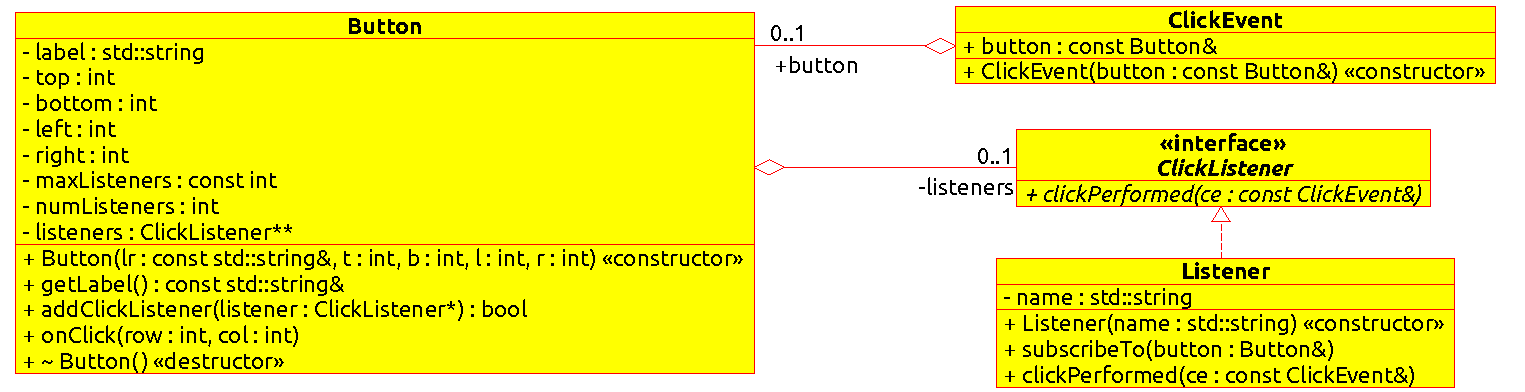
\includegraphics[scale=0.54]{interface.eps}
    \end{center}
\end{frame}

\begin{frame}
    \begin{exampleblock}{\textattachfile{ClickEvent.h}{ClickEvent.h}}
        \scriptsize
        \vspace{-.2cm}
        \lstinputlisting[language=C++,linerange={4-10},numbers=left,firstnumber=4]{ClickEvent.h}
        \vspace{-.2cm}
    \end{exampleblock}
    \begin{exampleblock}{\textattachfile{ClickListener.h}{ClickListener.h}}
        \scriptsize
        \vspace{-.2cm}
        \lstinputlisting[language=C++,linerange={4-9},numbers=left,firstnumber=4]{ClickListener.h}
        \vspace{-.2cm}
    \end{exampleblock}
\end{frame}

\begin{frame}
    \begin{exampleblock}{\textattachfile{Listener.h}{Listener.h}}
        \scriptsize
        \vspace{-.2cm}
        \lstinputlisting[language=C++,linerange={4-19},numbers=left,firstnumber=4]{Listener.h}
        \vspace{-.2cm}
    \end{exampleblock}
\end{frame}

\begin{frame}
    \begin{exampleblock}{\textattachfile{Button.h}{Button.h}}
        \scriptsize
        \vspace{-.2cm}
        \lstinputlisting[language=C++,linerange={7-22},numbers=left,firstnumber=7]{Button.h}
        \vspace{-.2cm}
    \end{exampleblock}
\end{frame}

\begin{frame}
    \begin{exampleblock}{\textattachfile{Button.h}{Button.h}}
        \small
        \vspace{-.2cm}
        \lstinputlisting[language=C++,linerange={23-31},numbers=left,firstnumber=23]{Button.h}
        \vspace{-.2cm}
    \end{exampleblock}
\end{frame}

\begin{frame}
    \begin{exampleblock}{\textattachfile{Button.cpp}{Button.cpp}}
        \scriptsize
        \vspace{-.2cm}
        \lstinputlisting[language=C++,linerange={1-17},numbers=left,firstnumber=1]{Button.cpp}
        \vspace{-.2cm}
    \end{exampleblock}
\end{frame}

\begin{frame}
    \begin{exampleblock}{\textattachfile{eventMain.cpp}{eventMain.cpp}}
        \footnotesize
        \vspace{-.2cm}
        \lstinputlisting[language=C++,linerange={1-14},numbers=left,firstnumber=1]{eventMain.cpp}
        \vspace{-.2cm}
    \end{exampleblock}
\end{frame}

\begin{frame}
    \begin{exampleblock}{\textattachfile{eventMain.cpp}{eventMain.cpp}}
        \scriptsize
        \vspace{-.2cm}
        \lstinputlisting[language=C++,linerange={15-22},numbers=left,firstnumber=15]{eventMain.cpp}
        \vspace{-.2cm}
    \end{exampleblock}
\end{frame}

\begin{frame}[fragile]
    \begin{block}{Kimenet}
        \vspace{-.3cm}
        \begin{verbatim}
row: 0
col: 0
Listener1 received a click event from Button1
Listener2 received a click event from Button1
row: 0
col: 150
Listener1 received a click event from Button2
row: 0
col: 300
row:     
        \end{verbatim}
        \vspace{-.6cm}
    \end{block}
\end{frame}

\subsection{Többszörös öröklődés}

\begin{frame}
    \begin{columns}[]
        \column{.8\textwidth}
            \begin{itemize}
                \item C++-ban létezik többszörös öröklődés (a legtöbb nyelv csak interfészekből enged többet megvalósítani, melyekre külön kulcsszó is van, pl. Java)
                \item Ha egy őstől több útvonalon is örököl egy leszármazott, nem lesz egyértelmű, melyiket kellene használni $\to$ virtuális öröklés
                      (vagy a probléma elodázása \texttt{::}-ral)
            \end{itemize}
        \column{.2\textwidth}
            \begin{center}
                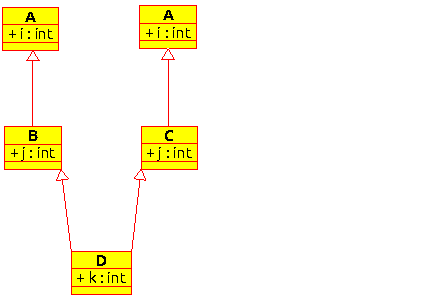
\includegraphics[scale=0.8]{diamond1.eps}
            \end{center}
    \end{columns}
\end{frame}

\begin{frame}
    \begin{columns}[T]
        \column{.5\textwidth}
            \begin{alertblock}{\textattachfile{diamond1.cpp}{diamond1.cpp}}
                \scriptsize
                \lstinputlisting[language=C++,linerange={1-14},numbers=left,firstnumber=1]{diamond1.cpp}
            \end{alertblock}
        \column{.5\textwidth}
            \begin{alertblock}{\textattachfile{diamond1.cpp}{}}
                \scriptsize
                \lstinputlisting[language=C++,linerange={16-26},numbers=right,firstnumber=16]{diamond1.cpp}
            \end{alertblock}
    \end{columns}
\end{frame}

\begin{frame}[fragile]
    \begin{block}{Kimenet}
        \vspace{-.3cm}
        \begin{verbatim}
diamond1.cpp: In function 'int main()':
diamond1.cpp:26:9: error: request for member 'i' is ambiguous
        obj.i = 42;
            ^
diamond1.cpp:5:9: note: candidates are: int A::i
        int i;
            ^
diamond1.cpp:5:9: note:                 int A::i   
        \end{verbatim}
        \vspace{-.6cm}
    \end{block}
\end{frame}

\begin{frame}
    \begin{columns}[]
        \column{.55\textwidth}
            \begin{exampleblock}{\textattachfile{diamond2.cpp}{diamond2.cpp}}
                \lstinputlisting[language=C++,linerange={6-14},numbers=left,firstnumber=6]{diamond2.cpp}
            \end{exampleblock}
        \column{.4\textwidth}
            \begin{center}
                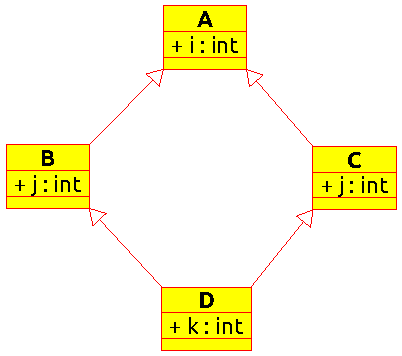
\includegraphics[scale=0.8]{diamond2.eps}
            \end{center}
    \end{columns}
\end{frame}